\documentclass[11pt]{charter}
\usepackage{rotating}
% El títulos de la memoria, se usa en la carátula y se puede usar el cualquier lugar del documento con el comando \ttitle
\titulo{ID Mobile - Sistema de identificación personal para teléfono móvil, mediante Bluetooth} 

% Nombre del posgrado, se usa en la carátula y se puede usar el cualquier lugar del documento con el comando \degreename
%\posgrado{Carrera de Especialización en Sistemas Embebidos} 
\posgrado{Carrera de Especialización en Internet de las Cosas} 
%\posgrado{Carrera de Especialización en Intelegencia Artificial}
%\posgrado{Maestría en Sistemas Embebidos} 
%\posgrado{Maestría en Internet de las cosas}

% Tu nombre, se puede usar el cualquier lugar del documento con el comando \authorname
\autor{Pedro Rosito} 

% El nombre del director y co-director, se puede usar el cualquier lugar del documento con el comando \supname y \cosupname y \pertesupname y \pertecosupname
\director{Nelson Fortunatti}
\pertenenciaDirector{ITBA} 
% FIXME:NO IMPLEMENTADO EL CODIRECTOR ni su pertenencia
\codirector{} % si queda vacio no se deberíá incluir 
\pertenenciaCoDirector{}

% Nombre del cliente, quien va a aprobar los resultados del proyecto, se puede usar con el comando \clientename y \empclientename
\cliente{Sergio Starkloff}
\empresaCliente{SURiX SRL}

% Nombre y pertenencia de los jurados, se pueden usar el cualquier lugar del documento con el comando \jurunoname, \jurdosname y \jurtresname y \perteunoname, \pertedosname y \pertetresname.
\juradoUno{Nombre y Apellido (1)}
\pertenenciaJurUno{pertenencia (1)} 
\juradoDos{Nombre y Apellido (2)}
\pertenenciaJurDos{pertenencia (2)}
\juradoTres{Nombre y Apellido (3)}
\pertenenciaJurTres{pertenencia (3)}
 
\fechaINICIO{25 de agosto de 2020}		%Fecha de inicio de la cursada de GdP \fechaInicioName
\fechaFINALPlanificacion{13 de octubre de 2020} 	%Fecha de final de cursada de GdP
\fechaFINALTrabajo{22 de julio de 2021}		%Fecha de defensa pública del trabajo final


\begin{document}

\maketitle
\thispagestyle{empty}
\pagebreak


\thispagestyle{empty}
{\setlength{\parskip}{0pt}
\tableofcontents{}
}
\pagebreak


\section{Registros de cambios}
\label{sec:registro}


\begin{table}[ht]
\label{tab:registro}
\centering
\begin{tabularx}{\linewidth}{@{}|c|X|c|@{}}
\hline
\rowcolor[HTML]{C0C0C0} 
Revisión & \multicolumn{1}{c|}{\cellcolor[HTML]{C0C0C0}Detalles de los cambios realizados} & Fecha      \\ \hline
1.0      & Creación del documento                                          & 25/08/2020 \\ \hline
1.1      & Se completó la descripción del proyecto & 2/09/2020 \\ \hline
1.2      & Se completaron parcialmente los puntos del 1 al 6 & 3/09/2020 \\ \hline
1.3		& Se terminó con los puntos del 1 al 6 y se completó la identificación y análisis de los interesados & 6/09/2020 \\ \hline
1.4     & Se agregaron las historias de usuario & 14/09/2020 \\ \hline
1.5		& Se realizaron correcciones y se completo hasta el punto 11 inclusive & 21/09/2020 \\ \hline
1.6     & Se finalizó con los puntos faltantes & 28/09/2020 \\ \hline
\end{tabularx}
\end{table}

\pagebreak



\section{Acta de constitución del proyecto}
\label{sec:acta}

\begin{flushright}
Buenos Aires, \fechaInicioName
\end{flushright}

\vspace{2cm}

Por medio de la presente se acuerda con el Ing. \authorname\hspace{1px} que su Trabajo Final de la \degreename\hspace{1px} se titulará ``\ttitle'', consistirá esencialmente en un sistema de identificación mobile utilizando tecnología Bluetooth, y tendrá un presupuesto preliminar estimado de 715 hs de trabajo y \textcolor{red}{\$XXX}, con fecha de inicio \fechaInicioName\hspace{1px} y fecha de presentación pública \fechaFinalName.

Se adjunta a esta acta la planificación inicial.

\vfill

% Esta parte se construye sola con la información que hayan cargado en el preámbulo del documento y no debe modificarla
\begin{table}[ht]
\centering
\begin{tabular}{ccc}
\begin{tabular}[c]{@{}c@{}}Ariel Lutenberg \\ Director posgrado FIUBA\end{tabular} & \hspace{2cm} & \begin{tabular}[c]{@{}c@{}}\clientename \\ \empclientename \end{tabular} \vspace{2.5cm} \\ 
\multicolumn{3}{c}{\begin{tabular}[c]{@{}c@{}} \supname \\ Director del Trabajo Final\end{tabular}} \vspace{2.5cm} \\
%\begin{tabular}[c]{@{}c@{}}\jurunoname \\ Jurado del Trabajo Final\end{tabular}     &  & \begin{tabular}[c]{@{}c@{}}\jurdosname\\ Jurado del Trabajo Final\end{tabular}  \vspace{2.5cm}  \\
%\multicolumn{3}{c}{\begin{tabular}[c]{@{}c@{}} \jurtresname\\ Jurado del Trabajo Final\end{tabular}} \vspace{.5cm}                                                                     
\end{tabular}
\end{table}




\section{Descripción técnica-conceptual del proyecto a realizar}
\label{sec:descripcion}

Surix es una empresa que se dedica al diseño y venta de porteros IP para el uso domiciliario, hospitalario y empresarial. 
Entre sus productos se destacan diferentes tipos de porteros, algunos de ellos presentan la posibilidad de manejarse mediante un celular con una aplicación llamada VoIPBell. Ésta aplicación tiene la limitación de poder manejar un sólo portero a la vez. \newline
Teniendo en cuenta que estamos frente a un contexto de cambio tecnológico en el mundo donde cada vez más servicios se pueden incluir en un celular y realizar de manera automatizada, se presenta un panoráma ideal para plantear avances en materia de comododiad funcional en aspectos de la vida diaria. \newline
Éste proyecto de ID Mobile viene a aportar la posibilidad de contar con una aplicación en la que los usuarios puedan crearse una cuenta mediante la cuál puedan tener acceso a todas las puertas en las que tengan instalado un portero Bluetooth, puede ser tanto de su casa como de su trabajo. Teniendo la posibilidad de programarlas, para que se abran a cierta hora de forma periódica, para dar acceso de única vez, para hacer control de rondas, entre otras funcionalidades. La aplicación propuesta se comunicará con un servidor el cuál tendrá acceso a una base de datos que almacenará las cuentas de los diferentes usuarios, ya sean administradores o usuarios llanos. A su vez la base de datos tendrá conocimiento, previa carga por parte del usuario, de todas las puertas Bluetooth instaladas de manera de poder asociarlas a los usuarios correspondientes. En la Figura 1 se muestra un diagrama de bloques en el que se puede observar el funcionamiento del sistema. 

\vspace{25px}

\begin{figure}[htpb]
\centering 
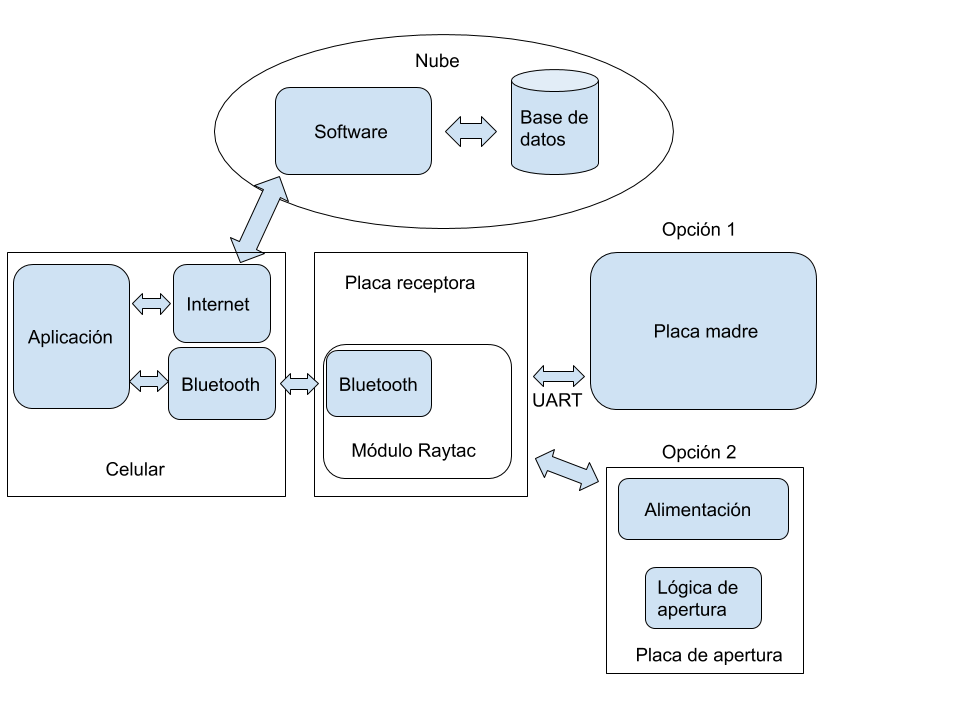
\includegraphics[width=.9\textwidth]{./Figuras/Diagramadebloques_planificacion.png}
\caption{Diagrama en bloques del sistema ID Mobile}
\label{fig:diagBloques}
\end{figure}

\vspace{25px}

Observamos en la figura que existen dos opciones, opción 1 y opción 2, esto se debe a que el sistema se comercializará como parte de un sistema mayor comandando por una placa madre (portero) que conocerá los permisos de cada usuario y en base a eso decidirá que acciones se deben llevar a cabo una vez recibida la señal por parte de la placa receptora (opción 1) o por otra parte el sistema se comercializará de forma standalone, es decir que existirá la placa receptora junto con la placa de apertura asociadas a una puerta y la aplicación será la que decida a partir de lo comunicado por el software en la nube si la puerta en cuestión puede o no abrirse (opción 2).



\section{Identificación y análisis de los interesados}
\label{sec:interesados}


\begin{table}[ht]
%\caption{Identificación de los interesados}
%\label{tab:interesados}
\begin{tabularx}{\linewidth}{@{}|l|X|X|l|@{}}
\hline
\rowcolor[HTML]{C0C0C0} 
Rol           & Nombre y Apellido & Organización 	& Puesto 	\\ \hline
Cliente       & \clientename      &\empclientename	& CTO       	\\ \hline
Responsable   & \authorname       & FIUBA        	& Alumno 	\\ \hline
Orientador    & \supname	      & \pertesupname 	& Director	Trabajo final \\ \hline
Colaborador        & Raúl Camacho      & SURiX SRL       & Desarrollador de software        	\\ \hline
\end{tabularx}
\end{table}


\begin{itemize}
\item Sergio Starkloff: No se encuentra actualmente en Argentina, pero a pesar de la diferencia horaria practicamente siempre está disponible para hacerle consultas. Está muy atento a todo lo referente al proyecto y siempre llega con nuevas propuestas e ideas. 
\item Nelson Fortunatti: Tiene mucho conocimiento de programación de microprocesadores por lo que su orientación será fundamental al momento de crear el software para la placa.
\item Raúl Camacho: Trabajaremos juntos en el diseño del hardware del proyecto, ya que es compartido con su trabajo de especialización.
\end{itemize}





\section{1. Propósito del proyecto}
\label{sec:proposito}


El propósito de éste proyecto es el de crear un sistema nuevo para la empresa, aprovechando la conectividad con la que cuentan prácticamente todos los celulares hoy en dia, abriendo la posibilidad de comenzar con una rama de productos orientada al internet de las cosas.


\section{2. Alcance del proyecto}
\label{sec:alcance}


En éste proyecto se incluye:
\begin{itemize}
\item El diseño de la placa receptora, utilizando un módulo previamente adquirido por la empresa, a través de un esquemático en Kicad.
\item El diseño de la placa de apertura, a través de un esquemático en Kicad.
\item La programación de un software en la placa receptora para la comunicación vía Bluetooth con un celular.
\item La creación de un software en aws (o algún servicio en la nube a determinar).
\item La creación de una base de datos en aws (o algún servicio en la nube a determinar).
\item La creación de una aplicación que pueda funcionar tanto en iOS como en Android.
\end{itemize}
En éste proyecto no se incluye:
\begin{itemize}
\item El diseño del pcb de las placas ni la implementación física de las mismas.
\item Ninguna etapa del diseño ni implementación de la placa madre.
\end{itemize}


\section{3. Supuestos del proyecto}
\label{sec:supuestos}

Para el desarrollo del presente proyecto se supone que:

\begin{itemize}
\item Las placas estarán implementadas en tiempo y forma para poder realizar las pruebas necesarias.
\item La programación de la aplicación que pueda funcionar en Android e iOS no será demasiado compleja para el tiempo estimado de realización de la tarea.
\item La complejidad de la programación del software para la placa receptora no será demasiado elevada para el tiempo estimado de realización de la tarea.
\item Será posible implementar todas las funciones requeridas para la aplicación.
\end{itemize}


\section{4. Requerimientos}
\label{sec:requerimientos}


\begin{enumerate}
\item Requerimientos asociados con la placa receptora.
	\begin{enumerate}
	\item Podrá comunicarse mediante Bluetooth con un celular.
	\item Será capaz de recibir alimentación y comunicarse mediante UART con una placa madre.
	\item Será capaz de recibir alimentación y comunicarse mediante 5 pines con una placa de apertura.
	\item Dispondrá de un jumper para cambiar de comportamiento para los dos casos anteriores.
	\item Podrá enviar una orden de apertura a la placa de apertura mediante un tren de pulsos.
	\item La lógica de apertura no podrá ser realizada de forma externa al sistema para evitar el vandalismo o robo.
	\end{enumerate}
\item Requerimientos asociados con la placa de apertura.
	\begin{enumerate}
	\item Será capaz de alimentar y comunicarse mediante 5 pines con la placa receptora.
	\item Podrá interpretar el tren de pulsos enviado por la placa receptora mediante un circuito contador o alguna lógica sencilla.
	\item Contará con un relé que se utilizará para abrir la puerta.
	\item Contará con una bocina para avisar de la apertura de la puerta.
	\item Podrá ser alimentada con 12V de alterna o continua.
	\end{enumerate}
\item Requerimientos asociados con la aplicación (mínimo producto viable)
	\begin{enumerate}
	\item Deberá ser capaz de comunicarse por Bluetooth con la placa receptora y mediante internet con el software en la nube.
	\item Deberá presentar una interfaz de usuario mediante la cuál gestionar el uso de las puertas disponibles.
	\item Deberá constituir un consumo muy bajo para la batería del celular.
	\item Se debe comunicar periódicamente con el software en la nube para revalidar permisos.
	\item La comunicación entre la aplicación y la placa receptora debe ser segura.
	\end{enumerate}
\item Requerimientos asociados con el sistema.
	\begin{enumerate}
	\item Debe funcionar en la nube (aws o alguna otra a determinar).
	\item Debe permitir a los usuarios crear una cuenta y asociarla a sus puertas.
	\item Debe permitir a los usuarios administrar sus puertas, cargándolas o eliminándolas del sistema, dando permisos a otros usuarios ya sea de forma periódica, de única vez o en franjas horarias determinadas.
	\item Debe permitir la configuración de la cuenta creada (cambiar foto, nombre, contraseña, etc.)
	\item Debe poder generar reportes de movimiento, tanto de usuarios como de cerraduras.
	\end{enumerate}
\end{enumerate}


\section{Historias de usuarios (\textit{Product backlog})}
\label{sec:backlog}

Ponderación: se puntúa según el esfuerzo que comprendería llevar a cabo la historia. El valor 1 representa el esfuerzo mínimo.

Prioridad: se puntúa del 1 al 5, donde el valor 1 representa lo más urgente.

Definimos usuario lock como el usuario dueño de puertas.

Definimos usuario key como el usuario que utiliza las puertas.

\begin{itemize}
\item Como usuario del sistema quiero acceder a una web para crear una cuenta.\textit{ Ponderación 5 - Prioridad 1} 
\item Como usuario del sistema quiero que exista una aplicación para crear una cuenta.\textit{ Ponderación 7 - Prioridad 4}
\item Como usuario del sistema quiero poder acceder a mi cuenta para modificar mis datos.\textit{ Ponderación 3 - Prioridad 2}
\item Como CTO de Surix quiero que exista una base de datos en la nube para que los usuarios puedan cargar sus puertas.\textit{ Ponderación 1 - Prioridad 1}
\item Como gestor de la base de datos quiero que exista un software en la nube para poder acceder a la base de datos.\textit{ Ponderación 3 - Prioridad 2}
\item Como usuario del sistema quiero que la aplicación sea multiplataforma para poder usarla en iOS y Android.\textit{ Ponderación 10 - Prioridad 5}
\item Como CTO de Surix quiero que exista una opción de gestión de cerraduras en el sistema para que los usuarios puedan añadir, quitar o asignar sus puertas.\textit{ Ponderación 5 - Prioridad 2}
\item Como usuario key del sistema quiero ver un listado de las puertas a las que tengo acceso para poder gestionarlas.\textit{ Ponderación 5 - Prioridad 1}
\item Como usuario lock del sistema quiero ver un listado de mis puertas para poder gestionarlas.\textit{ Ponderación 5 - Prioridad 1}
\item Como usuario del sistema quiero que la aplicación requiera de poca energía para que no me consuma rápidamente la batería del celular.\textit{ Ponderación 7 - Prioridad 2}
\item Como usuario del sistema quiero que la comunicación entre la aplicación y la puerta sea segura para evitar el vandalismo o robo.\textit{ Ponderación 7 - Prioridad 2}
\item Como CTO de Surix quiero que los usuarios reciban un mail de confirmación al crear su cuenta para añadir seguridad al sistema.\textit{ Ponderación 3 - Prioridad 5}
\item Como CTO de Surix quiero que el hardware creado sea compatible con el hardware utilizado por la empresa para evitar problemas de integración.\textit{ Ponderación 3 - Prioridad 1}
\item Como CTO de Surix quiero que las cuentas creadas tengan conexión entre ellas para que los usuario lock puedan dar acceso a los usuarios key.\textit{ Ponderación 7 - Prioridad 1}
\item Como usuario del sistema quiero que que la aplicación esté siempre actualizada con la base de datos para no tener problemas de acceso a mis puertas.\textit{ Ponderación 5 - Prioridad 2}
\item Como CTO de Surix quiero que la placa receptora envíe una orden de apertura a la placa de apertura para poder abrir la puerta.\textit{ Ponderación 7 - Prioridad 1}
\item Como CTO de Surix quiero que la aplicación se comunique con la placa receptora mediante Bluetooth, para que le pueda enviar los datos de identificación.\textit{ Ponderación 10 - Prioridad 1}
\item Como usuario del sistema quiero que la aplicación funcione en segundo plano para que no interrumpa otros usos del celular.\textit{ Ponderación 7 - Prioridad 2}


\end{itemize}

\section{5. Entregables principales del proyecto}
\label{sec:entregables}

\begin{itemize}
\item Esquemático de las placas receptora y de apertura.
\item Aplicación funcional para Android e iOS.
\item Software para la placa receptora que cumpla con los requerimientos especificados.
\item Software y base de datos en la nube.
\item Repositorio con el código fuente utilizado.
\item Documentación referente al código creado.

\end{itemize}


\section{6. Desglose del trabajo en tareas}
\label{sec:wbs}


\begin{enumerate}
\item Planificación del proyecto (60 hs)
	\begin{enumerate}
	\item Reuniones con el cliente para acordar los diferentes puntos. (5 hs)
	\item Estudio de los requerimientos planteados por el cliente (15 hs)
	\item Creación de la documentación. (40 hs)
	\end{enumerate}
\item Investigación previa (100 hs)
	\begin{enumerate}
	\item Estudio del módulo MDBT42Q de Raytac. (20 hs)
	\item Estudio y preparación del SDK de Nordic para el desarrollo del software en placa. (20 hs)
	\item Estudio sobre programación en la nube. (20 hs)
	\item Estudio sobre el protocolo de comunicación Bluetooth. (20 hs)
	\item Estudio sobre la programación de aplicaciones híbridas. (20hs)
	\end{enumerate}
\item Selección de recursos a utilizar (55 hs)
	\begin{enumerate}
	\item Selección de la nube de alguna compañia. (10 hs)
	\item Selección de componentes para el diseño de las placas. (15 hs)
	\item Selección de los lenguajes de programación a utilizar. (15 hs)
	\item Selección de los entornos de trabajo para la realización del software. (15 hs)
	\end{enumerate}
\item Desarrollo del hardware (100 hs)
	\begin{enumerate}
	\item Diseño de la lógica para la apertura de la puerta (20 hs)
	\item Realización del esquemático de la placa receptora. (40 hs)
	\item Realización del esquemático de la placa de apertura. (40 hs)
	\end{enumerate}
\item Desarrollo del software (295 hs)
	\begin{enumerate}
	\item Desarrollo del software en la nube (65 hs)
		\begin{enumerate}
		\item Desarrollo de la interfaz principal de usuario. (10 hs)
		\item Desarrollo de la interfaz y funcionalidad para la creación de cuenta. (15 hs)
		\item Desarrollo de la interfaz y funcionalidad para la configuración de cuenta. (25 hs)
		\item Desarrollo de la comunicación con la base de datos. (15 hs)
		\end{enumerate}
	\item Desarrollo de la aplicación (140 hs)
		\begin{enumerate}
		\item Desarrollo de la interfaz principal de usuario. (20 hs)
		\item Comunicación con Bluetooth para Android e iOS. (30 hs)
		\item Desarrollo de la interfaz y funcionalidad para la creación de cuenta. (20 hs)
		\item Desarrollo de la interfaz y funcionalidad para la configuración de cuenta. (30 hs)
		\item Integración y depuración del código para su funcionamiento tanto en Android como en iOS. (40 hs)
		\end{enumerate}
	\item Implementación de la base de datos en la nube. (30 hs)
	\item Desarrollo del software en la placa receptora. (60 hs)
	\end{enumerate}
\item Pruebas de integración (105 hs)
	\begin{enumerate}
	\item Implementación de la comunicación entre el software en la nube y la aplicación. (35 hs)
	\item Implementación de la comunicación vía Bluetooth entre el software en la placa y la aplicación. (35 hs)
	\item Implementación y pruebas del sistema completo. (35 hs)
	\end{enumerate}
	
\end{enumerate}

Cantidad total de horas: (715 hs)


\section{7. Diagrama de Activity On Node}
\label{sec:AoN}


\begin{figure}[htpb]
\centering 
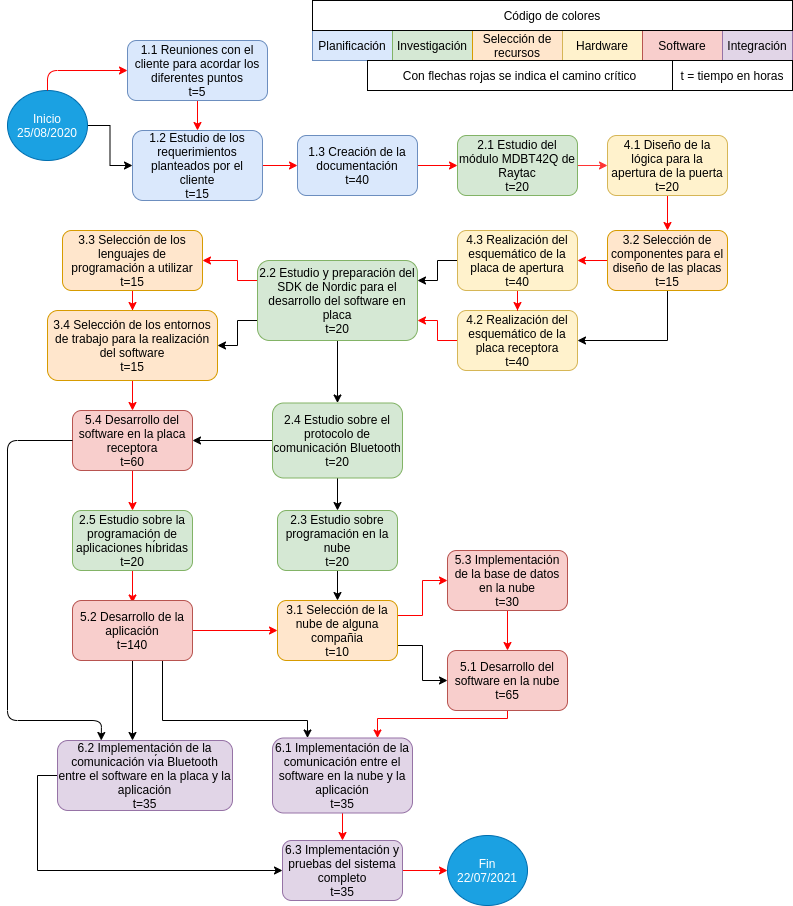
\includegraphics[width=.9\textwidth]{./Figuras/Aon2.png}
\caption{Diagrama en \textit{Activity on Node}}
\label{fig:AoN}
\end{figure}


\begin{itemize}
\item El camino crítico lleva un total de 640 horas.
\item Si la tarea 2.4 lleva más tiempo del estipulado, el camino que pasa por la misma hacia la 5.4 se convertiría en crítico.
\end{itemize}



\section{8. Diagrama de Gantt}
\label{sec:gantt}


\begin{figure}[htbp]
\centering
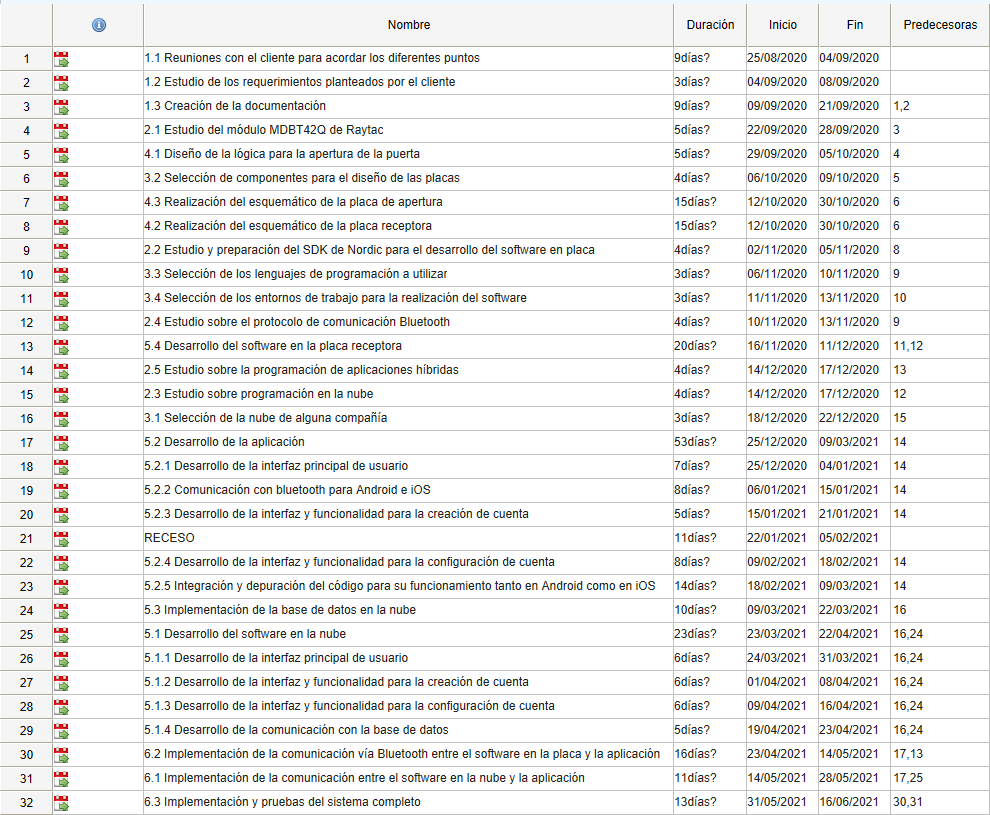
\includegraphics[width=1\textwidth]{./Figuras/DdG (2).png}
\caption{Cuadro diagrama de gantt}
\label{fig:gantt}
\end{figure}

\begin{figure}[htbp]

\centering
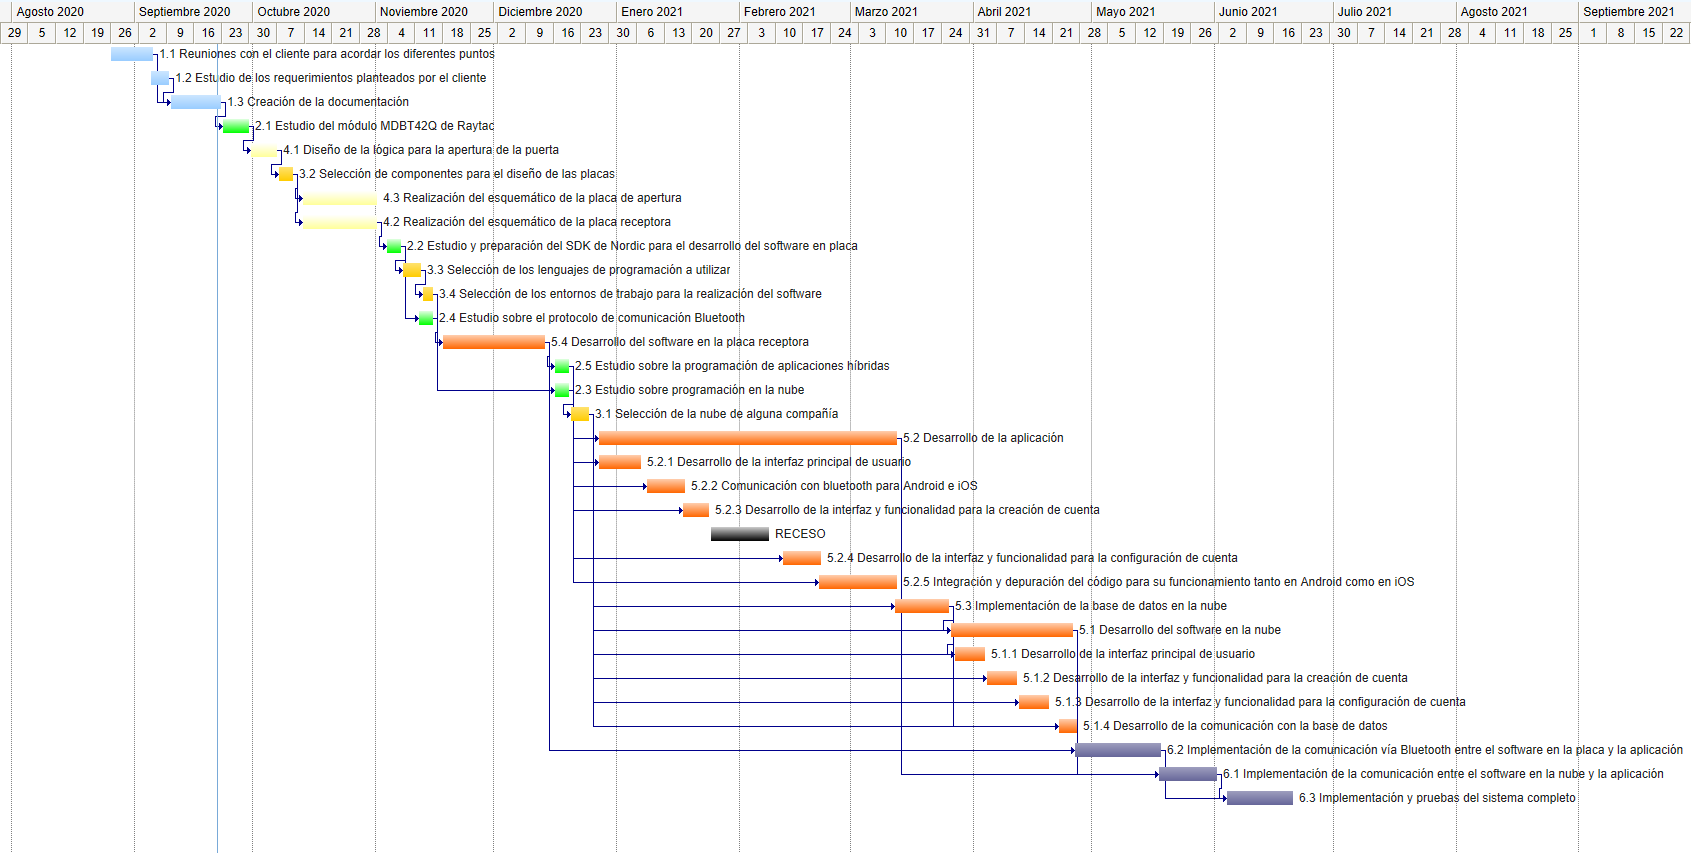
\includegraphics[width=1.5\textwidth , angle=90]{./Figuras/DdG (1).png}
\caption{Diagrama de gantt}
\label{fig:gantt}
\end{figure}

\section{9. Matriz de uso de recursos de materiales}
\label{sec:recursos}



\begin{table}[h!]
\label{tab:recursos}
\centering
\begin{tabularx}{\linewidth}{@{}|c|X|c|c|c|c|c|c|c|@{}}
\hline
\cellcolor[HTML]{C0C0C0} & \cellcolor[HTML]{C0C0C0} & \multicolumn{7}{c|}{\cellcolor[HTML]{C0C0C0}Recursos requeridos (horas)} \\ \cline{3-9} 
\multirow{-2}{*}{\cellcolor[HTML]{C0C0C0}\begin{tabular}[c]{@{}c@{}}Código\\ WBS\end{tabular}} & \multirow{-2}{*}{\cellcolor[HTML]{C0C0C0}\begin{tabular}[c]{@{}c@{}}Nombre \\ tarea\end{tabular}}& PC & Kicad & VS Code & SimulIDE & AWS & \begin{tabular}[c]{@{}c@{}}Placa\\ MDBT42Q \\ y J-link \end{tabular} & Celular  \\ \hline
 1& Planificación & 60 & - & - & - & - & - & -  \\ \hline
 2& Estudio & 90 & - & 10 & - & - & - & - \\ \hline
 3& Selección de recursos & 45 & - & - & - & - & -& - \\ \hline
 4.1&Diseño de la lógica para la apertura de la puerta  & - & - & - & 20 & - & - & -\\ \hline
 4.2& Diseño del esquemático de la placa receptora   & - &  20 & - & - & - & - & - \\ \hline
 4.3& Realización del esquemático de la placa de apertura & - &  20 & - & - & - & - & - \\ \hline
 5.1& Desarrolo del software en la nube  & - & - & 30 & - & 35 & -  & -\\ \hline
 5.2& Desarrollo de la aplicación & - & - & 120 & - & - & - & 20\\ \hline 
 5.3& Impl. de la base de datos en la nube & - & - & 15 & - & 15 & - & -\\ \hline
 5.4& Desarrollo del software en la placa receptora & - & - &  40 & - & - & 20 & -  \\ \hline
6& Pruebas de integración& - & - & 60 & - & 20 & 20 & 5 \\ \hline


\end{tabularx}%
\end{table}
 \newpage


\section{10. Presupuesto detallado del proyecto}
\label{sec:presupuesto}


\begin{table}[htpb]
\centering
\begin{tabularx}{\linewidth}{@{}|X|c|r|r|@{}}
\hline
\rowcolor[HTML]{C0C0C0} 
\multicolumn{4}{|c|}{\cellcolor[HTML]{C0C0C0}COSTOS DIRECTOS} \\ \hline
\rowcolor[HTML]{C0C0C0} 
Descripción &
  \multicolumn{1}{c|}{\cellcolor[HTML]{C0C0C0}Cantidad} &
  \multicolumn{1}{c|}{\cellcolor[HTML]{C0C0C0}Valor unitario} &
  \multicolumn{1}{c|}{\cellcolor[HTML]{C0C0C0}Valor total} \\ \hline
 Horas de ingeniero jr&
  \multicolumn{1}{c|}{715} &
  \multicolumn{1}{c|}{\$563} &
  \multicolumn{1}{c|}{\$402545} \\ \hline
 Placa MDBT42Q&
  \multicolumn{1}{c|}{1} &
  \multicolumn{1}{c|}{\$1432.62} &
  \multicolumn{1}{c|}{\$1432.62} \\ \hline
   SEGGER J-Link&
  \multicolumn{1}{c|}{1} &
  \multicolumn{1}{c|}{\$30363.23} &
  \multicolumn{1}{c|}{\$30363.23} \\ \hline
  Componentes electrónicos varios&
  \multicolumn{1}{c|}{-} &
  \multicolumn{1}{c|}{-} &
  \multicolumn{1}{c|}{\$1130.1} \\ \hline
   Diseño y fabricación del pcb&
  \multicolumn{1}{c|}{2} &
  \multicolumn{1}{c|}{\$8000} &
  \multicolumn{1}{c|}{\$16000} \\ \hline
  Montaje del prototipo&
  \multicolumn{1}{c|}{2} &
  \multicolumn{1}{c|}{\$760} &
  \multicolumn{1}{c|}{\$1520} \\ \hline
\multicolumn{3}{|c|}{SUBTOTAL} &
  \multicolumn{1}{c|}{\$452990.95} \\ \hline
\rowcolor[HTML]{C0C0C0} 
\multicolumn{4}{|c|}{\cellcolor[HTML]{C0C0C0}COSTOS INDIRECTOS} \\ \hline
\multicolumn{3}{|c|}{30\% de los costos directos} &
  \multicolumn{1}{c|}{\$135897.28} \\ \hline
\multicolumn{3}{|c|}{SUBTOTAL} &
  \multicolumn{1}{c|}{\$135897.28} \\ \hline
\rowcolor[HTML]{C0C0C0}
\multicolumn{3}{|c|}{TOTAL} & \$588888.23
   \\ \hline
\end{tabularx}%
\end{table}

Aclaraciones:
\begin{itemize}
\item La empresa es la encargada de realizar todas las compras y también es la encargada de realizar las contrataciones para los diseños necesarios que no fueron pactados para este proyecto, por lo que los costos mostrados son estimativos.
\item Para detallar algunos de los costos anteriores en pesos argentinos, se utilizó la cotización del dólar estadounidense a \$75,6.
\end{itemize}

\newpage

\section{11. Matriz de asignación de responsabilidades}
\label{sec:responsabilidades}


\begin{table}[h!]
\centering
\begin{tabularx}{\linewidth}{|c|X|c|c|c|c|}
\hline
\rowcolor[HTML]{C0C0C0} 
\cellcolor[HTML]{C0C0C0}\begin{tabular}[c]{@{}c@{}}Código\\ WBS\end{tabular} & 
\cellcolor[HTML]{C0C0C0}\begin{tabular}[c]{@{}c@{}}Nombre \\ tarea\end{tabular} & 
\begin{tabular}[c]{@{}c@{}} Responsable \\ \authorname \end{tabular}  & \begin{tabular}[c]{@{}c@{}} Orientador \\ \supname \end{tabular} & \begin{tabular}[c]{@{}c@{}} Colaborador \\ Raúl Camacho \end{tabular} & \begin{tabular}[c]{@{}c@{}} Cliente \\ \clientename \end{tabular} \\ \hline
      1 & Planificación & P  &  A   &   & I    \\ \hline
      2 & Estudio  & P  &  C   &   &    \\ \hline
      3 & Selección de recursos  & P  &  C   &  S & A     \\ \hline
      4.1 & Diseño de la lógica para la apertura de la puerta  & P  &  C   &   C & A    \\ \hline
      4.2 & Realización del esquemático de la placa receptora & P & C & P & A \\ \hline
      4.3 & Realización del esquemático de la placa de apertura & P  &  C   &  S & A   \\ \hline
      5.1 & Desarrollo del software en la nube & P & I & & A \\ \hline
      5.2 & Desarrollo de la aplicación & P & I & & A \\ \hline
      5.3 & Impl. de la base de datos en la nube & P & I & & A \\ \hline
      5.4 & Desarrollo del software en la placa receptora & P & C & C & A \\ \hline
      6 & Pruebas de integración & P & C & C & A \\ \hline

\end{tabularx}%
\end{table}




\section{12. Gestión de riesgos}
\label{sec:riesgos}

a) Identificación de los riesgos (al menos cinco) y estimación de sus consecuencias:
 
Riesgo 1: No llegar a cumplir con los tiempos especificados en el plan de proyecto.
\begin{itemize}
\item Severidad (S): 9. Ya que no se podría cumplir con el tiempo de entrega pactado para el cliente ni con el tiempo de finalización estipulado para la especialización.
\item Probabilidad de ocurrencia (O): 3. Debido a que sólo realizo el trabajo para la empresa y dispongo de tiempo para dedicarle.
\end{itemize}   

Riesgo 2: Que existan fallas en los componentes que me serán entregados para la programación de la placa.
\begin{itemize}
\item Severidad (S): 7. Dado a que me retrasaría en el comienzo del desarrollo del software en placa. 
\item Ocurrencia (O): 2. Los componentes son probados antes de ser enviados por lo que es poco probable que suceda.
\end{itemize}

Riesgo 3: Que se pierda el código de la aplicación.
\begin{itemize}
\item Severidad (S): 9. De perderse el código se atrazaría el proyecto un tiempo considerable.
\item Ocurrencia (O): 3. Es poco probable que suceda ya que implicaría algún desperfecto en el disco de la pc en la que está guardado o algún descuido grave.
\end{itemize}

Riesgo 4: Imposibilidad de realizar alguna de las instalaciones o alguna de las conexiones pertinentes para la programación.
\begin{itemize}
\item Severidad (S): 8. Cualquier inconveniente de este tipo conllevaría tiempo intentando buscar soluciones o caminos alternativos.
\item Ocurrencia (O): 7. Es sabido que al comenzar a trabajar con nuevas tecnologías pueden ocurrir inconvenientes de este tipo.
\end{itemize}

Riesgo 5: Que los prototipos de las placas receptora y de apertura tarden más de lo estipulado en ser fabricados.
\begin{itemize}
\item Severidad (S): 6. Se atrasaría la etapa final de pruebas del proyecto.
\item Ocurrencia (O): 3. La empresa tiene fabricantes de confianza que cumplen con los tiempos de entrega.
\end{itemize}

Riesgo 6: Problemas de comunicación con el cliente.
\begin{itemize}
\item Severidad (S): 9. Podría llevar a una mala interpretación de alguno de los requerimientos planteados y por ende a una incorrecta implementación del mismo.
\item Ocurrencia (O): 2. Se mantiene una comunicación fluida con el cliente por lo que no se espera que se tengan éste tipo de problemas.
\end{itemize}

Riesgo 7: Algún problema de compatibilidad entre el celular y la placa.
\begin{itemize}
\item Severidad (S): 10. Significaría un problema que haría que el proyecto no se pueda realizar tal y como está planteado.
\item Ocurrencia (O): 2. La comunicación entre el celular y la placa se realiza mediante bluetooth y está comprobado que es posible llevarla a cabo por lo que la probabilidad de ocurrencia es baja.
\end{itemize}

Riesgo 8: No contar con la colaboración del Ing. de Surix a tiempo para la realización de los esquemáticos.
\begin{itemize}
\item Severidad (S): 7. Llevaría a un retraso en la realización de los esquemáticos.
\item Ocurrencia (O): 2. Se pactaron los tiempos de trabajo con el Ing. en cuestión y se sabe que es responsable. 
\end{itemize}




b) Tabla de gestión de riesgos:      (El RPN se calcula como RPN=SxO)

\begin{table}[htpb]
\centering
\begin{tabularx}{\linewidth}{@{}|X|X|X|X|X|X|X|@{}}
\hline
\rowcolor[HTML]{C0C0C0} 
Riesgo & S & O & RPN & S* & O* & RPN* \\ \hline
    1  & 9 & 3 & \cellcolor[HTML]{F33B01} 27 &  9  &  2  & \cellcolor[HTML]{4EF301} 18     \\ \hline
    2  & 7 & 2 & \cellcolor[HTML]{4EF301} 14 &  -  &  -  & -     \\ \hline
    3  & 9 & 3 & \cellcolor[HTML]{F33B01} 27 &  9  &  1  &\cellcolor[HTML]{4EF301} 9     \\ \hline
    4  & 8 & 7 & \cellcolor[HTML]{F33B01} 56 &  10  & 2   & \cellcolor[HTML]{4EF301} 20     \\ \hline
    5  & 6 & 3 & \cellcolor[HTML]{4EF301} 18 &  -  & -   & -     \\ \hline
    6  & 9 & 2 & \cellcolor[HTML]{4EF301} 18 &  -  & -   & -     \\ \hline
    7  & 10 & 2 & \cellcolor[HTML]{4EF301}20 &  -  &  -  &   -   \\ \hline
    8  & 7 & 2 & \cellcolor[HTML]{4EF301} 14 &  -  &  -  &   -   \\ \hline
\end{tabularx}%
\end{table}

Criterio adoptado: 
Se tomarán medidas de mitigación en los riesgos cuyos números de RPN sean mayores a 25.

Nota: los valores marcados con (*) en la tabla corresponden luego de haber aplicado la mitigación.

c) Plan de mitigación de los riesgos que originalmente excedían el RPN máximo establecido:
 
Riesgo 1: No llegar a cumplir con los tiempos especificados en el plan de proyecto.
\begin{itemize}
\item Plan de mitigación: Ponerse metas semanales siguiendo el plan de trabajo establecido y realizar una verificación del cumplimiento de las mismas.
	\begin{itemize}
	\item Severidad (S): 9. La severidad se mantiene ya que de no cumplir con los tiempos se seguiría estando en falta con el cliente e incumpliendo los tiempos pactados para la especialización.
	\item Ocurrencia (O): 2. Al ponerse metas semanales y hacer un seguimiento de las mismas, junto con el plan de trabajo ya estipulado, el proyecto debería terminarse en tiempo y forma.
	\end{itemize}
\end{itemize}

Riesgo 3: Que se pierda el código realizado para el sistema.
\begin{itemize}
\item Plan de mitigación: Realizar un backup del código en un repositorio github y en google drive.
	\begin{itemize}
	\item Severidad (S): 9. La severidad no cambia ya que implicaría de igual modo un atraso de tiempo importante para el proyecto.
	\item Ocurrencia (O): 1. Al tener múltiples backups las posibilidades de que se dañen o por cualquier motivo se pierdan todos en simultáneo es muy poco probable.
	\end{itemize}
\end{itemize}
 
Riesgo 4: Imposibilidad de realizar la instalación y conexionado para la programación de la placa receptora.
\begin{itemize}
\item Plan de mitigación: Estudiar previamente el proceso de instalación y conexionado e identificar en que puntos pueden surgir problemas para buscar soluciones alternativas con antelación. 
	\begin{itemize}
	\item Severidad (S): 10. Si aún estudiando previamente y teniendo un plan secundario para el caso de fallas no se consigue lo buscado, podría llevar a que el proyecto no pueda continuar tal y como está planteado.
	\item Ocurrencia (O): 2. Es poco probable ya que existe abundante documentación respecto al módulo utilizado y múltiples maneras de realizar la programación del mismo.
	\end{itemize}
\end{itemize}


\section{13. Gestión de la calidad}
\label{sec:calidad}

\begin{enumerate}
\item Requerimientos asociados con la placa receptora.
	\begin{enumerate}
	\item Podrá comunicarse mediante Bluetooth con un celular.
		\begin{itemize}
		\item Verificación: Análisis de las hojas de datos del módulo MDBT42Q y estudio del protocolo de comunicación Bluetooth. 
		\item Validación: Constatar una vez programada la placa que puede realizarse la comunicación mediante bluetooth con un celular.
		\end{itemize}

	\item Será capaz de recibir alimentación y comunicarse mediante UART con una placa madre.
		\begin{itemize}
		\item Verificación: Análisis de las hojas de datos del módulo MDBT42Q y de la comunicación mediante UART. 
		\item Validación: Una vez creado el prototipo de la placa, verificar que recibe alimentación y se comunica mediante UART con la placa madre.
		\end{itemize}

	\item Será capaz de recibir alimentación y comunicarse mediante 5 pines con una placa de apertura.
		\begin{itemize}
		\item Verificación: Análisis de las hojas de datos del módulo MDBT42Q.
		\item Validación: Una vez creado el prototipo de la placa, verificar que recibe alimentación y se comunica mediante 5 pines con la placa de apertura.
		\end{itemize}
	
	\item Dispondrá de un jumper para cambiar de comportamiento para los dos casos anteriores.
		\begin{itemize}
		\item Verificación: Análisis de las hojas de datos del módulo MDBT42Q.
		\item Validación: Constatar una vez creado el prototipo que mediante el uso de un jumper se puede cambiar el comportamiento respecto al uso de UART o 5 pines.
		\end{itemize}
	
	\item Podrá enviar una orden de apertura a la placa de apertura mediante un tren de pulsos.
		\begin{itemize}
		\item Verificación: Análisis de las hojas de datos del módulo MDBT42Q.
		\item Validación: Constatar mediante la programación de la placa que es capaz de enviar un tren de pulsos.
		\end{itemize}
		
			\item La lógica de apertura no podrá ser realizada de forma externa al sistema para evitar el vandalismo o robo.
		\begin{itemize}
		\item Verificación: Análisis de las hojas de datos del módulo MDBT42Q y del esquemático de la placa.
		\item Validación: Constatar una vez creado el prototipo que no es posible realizar la lógica de apertura si no es a través de un celular con la aplicación adecuada.
		\end{itemize}
	\end{enumerate}
	
\item Requerimientos asociados a la placa de apertura.
	\begin{enumerate}
	\item Será capaz de alimentar y comunicarse mediante 5 pines con la placa receptora.
		\begin{itemize}
		\item Verificación: Análisis del esquemático de la placa y de las hojas de datos de los componentes utilizados. 
		\item Validación: Una vez creado el prototipo verificar que es capaz de comunicarse mediante 5 pines con la placa receptora.
		\end{itemize}

	\item Podrá interpretar el tren de pulsos enviado por la placa receptora mediante un circuito contador o alguna lógica sencilla.
		\begin{itemize}
		\item Verificación: Análisis de la hoja de datos del contador 74LS90 y simulación del circuito de apertura mediante software en la PC.
		\item Validación: Una vez creado el prototipo de la placa verficar si es capaz de interpretar el tren de pulsos enviado por la placa receptora.
		\end{itemize}

	\item Contará con un relé que se utilizará para abrir la puerta.
		\begin{itemize}
		\item Verificación: Estudio del esquemático implementado para la placa.
		\item Validación: Una vez creado el prototipo verificar que el mismo cuenta con un relé.
		\end{itemize}
	
	\item Contará con una bocina para avisar de la apertura de la puerta.
		\begin{itemize}
		\item Verificación: Estudio del esquemático implementado para la placa.
		\item Validación: Una vez creado el prototipo verificar que el mismo cuenta con una bocina en paralelo con el relé.
		\end{itemize}
	
	\item Podrá ser activada con 12V de alterna o continua.
		\begin{itemize}
		\item Verificación: Estudio del esquemático implementado para la placa.
		\item Validación: Una vez creado el prototipo de la placa verificar que puede ser alimentada con 12V de alterna o continua.
		\end{itemize}
		
	\end{enumerate}
\item Requerimientos asociados con la aplicación (mínimo producto viable).	
	\begin{enumerate}
	\item Deberá ser capaz de comunicarse por Bluetooth con la placa receptora y mediante internet con el software en la nube.
		\begin{itemize}
		\item Verificación: Análisis del código de la aplicación y de los protocolos de comunicación involucrados.
		\item Validación: Una vez finalizados los códigos de comunicación verificar que cumplen con lo propuesto.
		\end{itemize}
		
	\item Deberá presentar una interfaz de usuario mediante la cuál gestionar el uso de las puertas disponibles.
		\begin{itemize}
		\item Verificación: Análisis del código de la aplicación.
		\item Validación: Una vez finalizada la etapa de interfaz con el usuario verificar que cuenta con la posibilidad de gestionar el uso de puertas.
		\end{itemize}
		
	\item Deberá constituir un consumo muy bajo para la batería del celular.
		\begin{itemize}
		\item Verificación: Análisis de los recursos que consumen los diferentes procesos a realizar por la aplicación.
		\item Validación: Constatar una vez finalizada la aplicación mediante una prueba de uso si efectivamente consume poca batería.
		\end{itemize}
		
	\item Se debe comunicar periódicamente con el software en la nube para revalidar permisos.
		\begin{itemize}
		\item Verificación: Análisis del código de la aplicación y del método de comunicación con la base de datos.
		\item Validación: Una vez finalizada la aplicación constatar que se comunica periódicamente con el software en la nube.
		\end{itemize}
		
		\item La comunicación entre la aplicación y la placa receptora debe ser segura.
		\begin{itemize}
		\item Verificación: Análisis del código de la aplicación y del protocolo de comunicación Bluetooth.
		\item Validación: Una vez finalizada la aplicación constatar que la comunicación de la misma con la placa se encuentra encriptada.
		\end{itemize}
	\end{enumerate}
	
\item Requerimientos asociados con el sistema.
	\begin{itemize}
	\item Verificación: Análisis del código creado para el software en la nube.
	\item Validación: Constatar una vez finalizado el sistema que cumple con los requerimientos especificados de funcionamiento y funcionalidades prestadas.
	\end{itemize}
	
\end{enumerate}

\newpage

\section{14. Comunicación del proyecto}
\label{sec:comunicaciones}

El plan de comunicación del proyecto es el siguiente:

\begin{table}[htpb]
\centering
\begin{tabularx}{\linewidth}{@{}|X|C{2.4cm}|C{3cm}|C{1.8cm}|C{2cm}|C{2.1cm}|@{}}
\hline
\rowcolor[HTML]{C0C0C0} 
\multicolumn{6}{|c|}{\cellcolor[HTML]{C0C0C0}PLAN DE COMUNICACIÓN DEL PROYECTO}           \\ \hline
\rowcolor[HTML]{C0C0C0} 
¿Qué comunicar? & Audiencia & Propósito & Frecuencia & Método de comunicac. & Responsable \\ \hline
       Plan de proyecto   &     Clase de gestión de proyectos, director de proyecto      &      Evaluación y aprobación del proyecto     &     Única vez (al inicio del proyecto)       &                 Correo electrónico y/o reunión &   Pedro Rosito          \\ \hline
       Avances del proyecto         &     Cliente, director de proyecto      &     Informar y solicitar aprobación o correcciones      &     Cada 15 días o mensual, dependiendo de los avances realizados       &          Correo electrónico y/o reunión            &     Pedro Rosito        \\ \hline
          Resolución de problemas y consultas      &     Cliente, director de proyecto      &     Informar y consultar para recibir recomendaciones      &      Cuando sea necesario      &                     Correo electrónico y/o reunión &     Pedro Rosito        \\ \hline
      Finalización del proyecto          &     Cliente, director y jurado      &     Presentación formal y cierre del proyecto      &     Uníca vez (al finalizar el proyecto)       &                     Correo electrónico, reunión y presentación formal &     Pedro Rosito        \\ \hline

\end{tabularx}
\end{table}

\section{15. Gestión de compras}
\label{sec:compras}

Todos los elementos necesarios para el desarrollo del proyecto tales como componentes electrónicos y la placa de desarrollo, así como la contratación de los servicios en la nube serán provistos y realizados por la empresa.

\newpage

\section{16. Seguimiento y control}
\label{sec:seguimiento}



\begin{table}[!htpb]
\centering
%\begin{tabularx}{\linewidth}{@{}|X|X|X|X|X|X|@{}}
\begin{tabularx}{\linewidth}{@{}|X|C{2.5cm}|C{3cm}|C{2cm}|C{2cm}|C{2.5cm}|@{}}
\hline
\rowcolor[HTML]{C0C0C0} 
\multicolumn{6}{|c|}{\cellcolor[HTML]{C0C0C0}SEGUIMIENTO DE AVANCE}                                                                       \\ \hline
\rowcolor[HTML]{C0C0C0} 
Tarea del WBS & Indicador de avance & Frecuencia de reporte & Resp. de seguimiento & Persona a ser informada & Método de comunic. \\ \hline
1 & Avance en la planificación  & Semanal & \authorname & \supname & Correo electrónico \\ \hline
2 & Cantidad de temas investigados & Cada 15 días & \authorname & \supname & Correo electrónico \\ \hline
3 & Cantidad de tareas para las cuáles se seleccionaron los recursos &Cada 15 días & \authorname & \supname ,  \clientename & Correo electrónico  \\ \hline
4 & Porcentaje de avance en las subtareas & Semanal & \authorname & \supname , \clientename & Correo electrónico \\ \hline
5 & Cantidad de funcionalidades implementadas & Semanal & \authorname & \supname , \clientename & Correo electrónico \\ \hline
6 & Porcentaje de integración del sistema & Semanal & \authorname & \supname , \clientename & Correo electrónico \\ \hline
\end{tabularx}%
%}
\end{table}

\section{17. Procesos de cierre}    
\label{sec:cierre}

Al finalizar el proyecto se seguirán los siguientes pasos:
\begin{itemize}
\item Reunión con el cliente. \\
Encargado: Pedro Rosito. \\
El encargado del proyecto presentará al cliente toda la documentación correspondiente y cualquier entregable faltante que se haya acordado al inicio del proyecto.
El proyecto será entonces evaluado según los siguientes criterios:
\begin{itemize}
\item Cumplimiento de los requerimientos establecidos.
\item Cumplimiento con los tiempos estipulados de finalización.
\end{itemize}
A su vez se evaluará al alumno según los siguientes criterios:
\begin{itemize}
\item Solvencia en la resolución del trabajo.
\item Comunicación con el cliente.
\end{itemize}
En base a las evaluaciones anteriores, en conjunto con el director del proyecto, se analizará, a partir del WBS y de la gestión de riesgos propuesta, que procedimientos llevados a cabo fueron útiles y cuáles inútiles. Teniendo en cuenta sobre todo, el tiempo empleado para la finalización del proyecto y el tiempo que se estipulaba emplear en un principio.
\item Presentación final del proyecto frente a los jurados. \\
Encargado: Pedro Rosito. \\
Se realizará una presentación formal del proyecto para los jurados y todos los interesados donde se agradecerá a los directores de la CEIoT, a los profesores y al director del proyecto.
\end{itemize}

\end{document}